\documentclass[]{article}
\newcommand{\FileDepth}{../../..}
\usepackage[letterpaper, landscape, margin=0.5cm]{geometry}
\usepackage[T1]{fontenc}
\usepackage{textcomp}%Not strictly necessary, but gives \textmu command for "micro."
\usepackage{fancyhdr}
\usepackage{amsmath}
\usepackage{amssymb}
\usepackage{graphicx}
\usepackage{xcolor}
\usepackage{tikz}
\usetikzlibrary{calc}
\usepackage[shortlabels]{enumitem}
\usepackage{multicol}
\usepackage{vwcol}
\usepackage{hyperref}
\usepackage{wrapfig}
%opening
\newcommand{\SecType}{L}
\newcommand{\Week}{15}
\title{PH 211 Lecture \Week}
\author{Benjamin Bauml}
\date{Summer 2024}

\newcommand{\Purpose}{4}
\newcommand{\DefOnly}{0}

\input{\FileDepth/Formats/Assignment20240614.tex}
\usepackage[absolute]{textpos}
% This package relies on Assignment Format 2024-06-14 or later to work. It is recommended that the Purpose and DefOnly commands be given as such:
%\newcommand{\Purpose}{4}
%\newcommand{\DefOnly}{0}
% Activities need to be entered outside of the TeacherMargin and PresentSpace environments, otherwise they will be defined only locally. They can even go in the preamble.
\newenvironment{TeacherMargin}{\begin{textblock*}{10.8cm}(0.5cm,0.5cm)
\small}{\end{textblock*}
\hspace{0.1cm}}
\newenvironment{PresentSpace}{\begin{textblock*}{0.3cm}(26.85cm,9.35cm)
--
\end{textblock*}
\begin{textblock*}{15.6cm}(11.8cm,0.5cm)
\begin{Repurpose}{1}
\Large}{\end{Repurpose}
\end{textblock*}
\hspace{0.1cm}}

\newcommand{\FBDaxes}[4][2]{
	\begin{scope}[shift={(#2)},rotate=#3]
		% x-axis
		\draw[thick,->] (-#1,0) -- (#1,0);
		\node[anchor=west] at (#1,0) {$x$};
		% y-axis
		\draw[thick,->] (0,-#1) -- (0,#1);
		\node[anchor=south] at (0,#1) {$y$};
		\coordinate (#4) at (0,0);
	\end{scope}
}
\newcommand{\FBDvectorMA}[4]{
	\begin{scope}[shift={(#1)}]
		\coordinate (#4tip) at ({#2*cos(#3)},{#2*sin(#3)});
		\draw[ultra thick,blue,->] (#1) -- (#4tip);
	\end{scope}
}
\newcommand{\FBDvectorXY}[3]{
	\begin{scope}[shift={(#1)}]
		\coordinate (#3tip) at (#2);
		\draw[ultra thick,blue,->] (0,0) -- (#3tip);
	\end{scope}
}
\newcommand{\FBDdot}[1]{
	\filldraw[black] (#1) circle (3pt);
}
\newcommand{\FBDbox}[5][1]{
	\begin{scope}[shift={(#2)},rotate=#3]
		\filldraw[color=black,fill=white,thick] ({-#1/2},{#1/2}) -- ({-#1/2},{-#1/2}) -- ({#1/2},{-#1/2}) -- ({#1/2},{#1/2}) -- cycle;
		% Left side coordinates
		\coordinate (#4ltq) at ({-#1/2},{#1/4});
		\coordinate (#4lcent) at ({-#1/2},0);
		\coordinate (#4lbq) at ({-#1/2},{-#1/4});
		% right side coordinates
		\coordinate (#4rtq) at ({#1/2},{#1/4});
		\coordinate (#4rcent) at ({#1/2},0);
		\coordinate (#4rbq) at ({#1/2},{-#1/4});
		% top coordinates
		\coordinate (#4tlq) at ({-#1/4},{#1/2});
		\coordinate (#4tcent) at (0,{#1/2});
		\coordinate (#4trq) at ({#1/4},{#1/2});
		% bottom coordinates
		\coordinate (#4blq) at ({-#1/4},{-#1/2});
		\coordinate (#4bcent) at (0,{-#1/2});
		\coordinate (#4brq) at ({#1/4},{-#1/2});
		% corners
		\coordinate (#4tl) at ({-#1/2},{#1/2});
		\coordinate (#4tr) at ({#1/2},{#1/2});
		\coordinate (#4bl) at ({-#1/2},{-#1/2});
		\coordinate (#4br) at ({#1/2},{-#1/2});
		\node at (0,0) {#5};
	\end{scope}
}
%\newcommand{\MVec}[3][0]{%Creates a momentum vector of length #3 centered at #2 and rotated #1 degrees counterclockwise.
	\begin{scope}[rotate=#1,shift={(#2)}]
		\draw[->,thick] ({-#3/2},0) -- ({#3/2},0);
	\end{scope}
}
\newcommand{\MDot}[1]{%Creates a dot at #1 to represent a zero vector.
	\filldraw (#1) circle (1pt);
}
\newcommand{\MVDRows}[2][4.5]{%Creates the rows (initial, delta, final) of a momentum vector diagram. The optional argument determines the width of the table, and defaults to a good length for three columns (two objects and the total system). The non-optional argument gives a coordinate name (not displayed) to the diagram.
	\begin{scope}
		%\draw[thick] (0,5.5) -- (0,0);
		\draw[thick] (-1,4.5) -- (#1,4.5);
		\node at (-0.5,3.75) {$\vec{p}_{i}$};
		\draw[thick] (-1,3) -- (#1,3);
		\node at (-0.5,2.25) {$\Delta\vec{p}$};
		\draw[thick] (-1,1.5) -- (#1,1.5);
		\node at (-0.5,0.75) {$\vec{p}_{f}$};
		\coordinate (#2) at (0,5);
	\end{scope}
}
\newcommand{\MVDCol}[4][0.75]{%Creates a column for an object in a momentum vector diagram. The first (non-optional) argument is the coordinate name (not displayed) of the column, while the second is the displayed column header. The first argument also names the three entries down the column. The third argument anchors the column, so it should either be the coordinate name of the MVD (for the first column) or the coordinate name of the previous column. The optional argument indicates how far the center of the column should be from the previous column's edge, and defaults to 0.75.
	\begin{scope}[shift={(#4)}]
		\node at (#1,0) {#3};
		%\draw[thick] ({#1*2},0.5) -- ({#1*2},-5);
		\draw[thick] (0,0.5) -- (0,-5);
		\coordinate (#2init) at (#1,-1.25);
		\coordinate (#2delt) at (#1,-2.75);
		\coordinate (#2fin) at (#1,-4.25);
		\coordinate (#2) at ({#1*2},0);
	\end{scope}
}

%\input{\FileDepth/Activities/Activity_One/Activity_One.tex}
%\input{\FileDepth/Activities/Activity_Two/Activity_Two.tex}

\begin{document}
\begin{TeacherMargin}
\noindent When placed tail to tail, vector (C) forms an obtuse (greater than 90 degrees) angle with the red vector. The dot product of two vectors $\vec{v}$ and $\vec{w}$ is
\[
\vec{v}\cdot\vec{w} = vw\cos\theta,
\]
where $\theta$ is the angle between the two vectors (when they are tail-to-tail). Angles greater than 90 degrees will make the dot product negative.
\end{TeacherMargin}
\begin{PresentSpace}
\begin{center}
	\huge Lecture \Week: Energy and Power
\end{center}
\vspace{0.5cm}
\underline{Warm-Up Activity} \\
Which of these vectors, when dotted with the red vector below, results in a negative value? \\
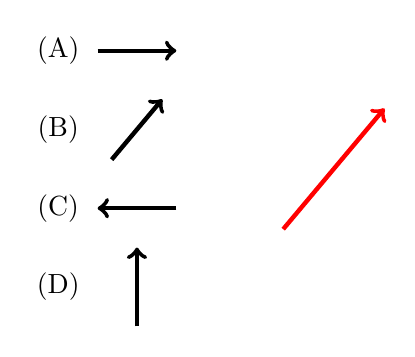
\begin{tikzpicture}
	\foreach \y in {1,2,3,4}
		\node (n\y) at (0,-\y) {};
	\begin{scope}[shift={(n1)}]
		\node at (-1,0) {(A)};
		\draw[ultra thick,->,rotate=0] (-0.5,0) -- (0.5,0);
	\end{scope}
	\begin{scope}[shift={(n2)}]
		\node at (-1,0) {(B)};
		\draw[ultra thick,->,rotate=50] (-0.5,0) -- (0.5,0);
	\end{scope}
	\begin{scope}[shift={(n3)}]
		\node at (-1,0) {(C)};
		\draw[ultra thick,->,rotate=180] (-0.5,0) -- (0.5,0);
	\end{scope}
	\begin{scope}[shift={(n4)}]
		\node at (-1,0) {(D)};
		\draw[ultra thick,->,rotate=90] (-0.5,0) -- (0.5,0);
	\end{scope}
	\draw[ultra thick,red,->,shift={(2.5,-2.5)},rotate=50] (-1,0) -- (1,0);
\end{tikzpicture}
\end{PresentSpace}
\newpage
\begin{TeacherMargin}
\noindent\textbf{Types of Energy} \\
The ball is in motion, so it has kinetic energy all to itself. During the bounce, the ball changes shape (deforms), which stores a form of potential energy (elastic potential energy).

There is another form of potential energy---gravitational potential energy---shared between the ball and the Earth. It belongs to neither of them individually.

Finally, collisions jostle molecules and produce heat, so there are separate stores of thermal energy in both the ball and the ground. \\
\textbf{Transformations} \\
As the ball falls, the gravitational potential energy it shares with the Earth is transformed into kinetic energy. During the collision, a lot of this energy becomes elastic potential energy as the ball squishes down and comes to a brief stop. There is technically a little change in gravitational potential energy, since the mass distributed in the ball moves as it squishes down. Some of the kinetic energy instead becomes thermal energy that is divided between the ball and the ground. After the bounce, the elastic potential energy has been converted back into kinetic energy (less than it had when it hit the ground) as the ball speeds upward again, gradually getting slower and slower as its kinetic energy returns to gravitational potential. \\
\textbf{Calculable} \\
We have the equations necessary to calculate work, and we could figure out the force of gravity and the displacement of the ball, so the work done by gravity is calculable. Through the work-energy theorem, we would then be able to calculate the change in its kinetic energy over the course of the fall. We could use the same techniques to find the kinetic energy after the collision from the ending height of the ball after the bounce. The difference from before and after the bounce would tell us how much was lost to thermal energy, though not how that energy was split between the ball and the ground.
\end{TeacherMargin}
\begin{PresentSpace}
\vspace{-10pt}
\section*{L\Week-1: The Drop and Bounce}
\vspace{-10pt}
You drop a tennis ball of the top of a tall building. It falls to the ground, bounces, and rises back into the air.
\begin{itemize}
	\item Identify the different types of energy in this situation and to which object or system these energies belong.
	\item Describe how energy is transformed within systems and transferred between systems during the drop and bounce.
	\item Which of the energies, transformations, or transfers do you think you might be able to calculate?
\end{itemize}
\end{PresentSpace}
\newpage
\begin{TeacherMargin}
\noindent\textbf{Work vs. Energy} \\
Energy is a property of a system that describes the system's capacity to exert forces that can impact the displacement of other systems. Work describes energy transfer between systems when done through forces. \\

\noindent\textbf{Coordinate System Care} \\
What if my path from the initial point to the final point goes in the negative direction of my coordinate system?
\begin{center}
	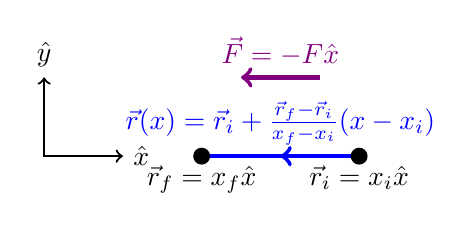
\begin{tikzpicture}
		\draw[thick,<->] (0,1) node[anchor=south] {$\hat{y}$} -- (0,0) -- (1,0) node[anchor=west] {$\hat{x}$};
		\draw[ultra thick,blue,->] (4,0) -- (3,0) node[anchor=south] {$\vec{r}(x) = \vec{r}_{i} + \frac{\vec{r}_{f}-\vec{r}_{i}}{x_{f}-x_{i}}(x-x_{i})$};
		\draw[ultra thick,blue] (3.1,0) -- (2,0);
		\filldraw (2,0) node[anchor=north] {$\vec{r}_{f}=x_{f}\hat{x}$} circle (0.1);
		\filldraw (4,0) node[anchor=north] {$\vec{r}_{i}=x_{i}\hat{x}$} circle (0.1);
		\draw[ultra thick,violet,->] (3.5,1) -- (3,1) node[anchor=south] {$\vec{F} = -F\hat{x}$} -- (2.5,1);
	\end{tikzpicture}
\end{center}
If force and displacement are in the same direction, the work should be positive, but how does this show up in the math?
\[
W = \int_{r_{i}}^{r_{f}}\vec{F}\cdot d\vec{r} = \int_{r_{i}}^{r_{f}}\vec{F}\cdot \frac{d\vec{r}}{dx}dx = -\int_{x_{i}}^{x_{f}} Fdx = \int_{x_{f}}^{x_{i}}Fdx > 0
\]
\[
\frac{d\vec{r}}{dx} = \frac{\vec{r}_{f}-\vec{r}_{i}}{x_{f}-x_{i}} = \frac{x_{f}\hat{x}-x_{i}\hat{x}}{x_{f}-x_{i}} = \frac{x_{f}-x_{i}}{x_{f}-x_{i}}\hat{x} = \hat{x}
\]
Because our path $\vec{r}(x)$ has the same length scale as our parameterization $x$, the derivative just gives us direction.

An easy mistake is to look at $W=\int_{x_{i}}^{x_{f}}\vec{F}\cdot d\vec{x}$, plug in
\[
W = \int_{x_{i}}^{x_{f}}(-F)(-dx) = \int_{x_{i}}^{x_{f}}Fdx = -\int_{x_{f}}^{x_{i}}Fdx,
\]
and get a negative work by accidentally introducing an extra negative sign. It is important to make a clear distinction between the path $\vec{r}(x)$ and the parameterization $x$.

Rather than fixate on the highly mathematical version, the basic takeaway from this is that you should either integrate the path from the larger $x_{i}$ to the smaller $x_{f}$ against the direction of $d\vec{x}$, or you should integrate from the smaller $x_{f}$ to the larger $x_{i}$ and introduce a negative sign ($-d\vec{x}$) to indicate the orientation of the path. Introducing both will cause problems.
\end{TeacherMargin}
\begin{PresentSpace}
\vspace{-10pt}
\section*{Changing a System's Energy}
\vspace{-10pt}
\begin{itemize}
	\item The total energy of a system can only change through an \textit{interaction} with something external to the system.
	\item If that interaction is a force, then the energy transferred to the system is known as \textit{work}.
	\[
	W = \int_{r_{i}}^{r_{f}}\vec{F}\cdot d\vec{r}
	\]
\end{itemize}
\end{PresentSpace}
\newpage
\begin{TeacherMargin}
Let the ball start at height $y_{i} = h$ and end at $y_{f}=0$. The work done by gravity is
\[
W = \int_{r_{i}}^{r_{f}}\vec{F}\cdot d\vec{r} = \int_{y_{i}}^{y_{f}}\vec{F}\cdot \frac{d\vec{r}}{dy} dy.
\]
Just like on the previous page, $\frac{d\vec{r}}{dy} = \hat{y}$, so
\[
W = \int_{h}^{0} (-mg\hat{y})\cdot(dy\hat{y}) = mg\int_{0}^{h}\hat{y}\cdot\hat{y}dy = mg\int_{0}^{h}dy = mgh.
\]
This does not depend on initial speed, only the distance it falls from its initial height, so it does not matter if you throw it! The works are equal.
\end{TeacherMargin}
\begin{PresentSpace}
\vspace{-10pt}
\section*{L\Week-2: The Drop -- Part 1}
\vspace{-10pt}
\begin{itemize}
	\item Consider the system of the tennis ball.
	\item Starting at the moment you drop the ball and ending right before the ball hits the ground:
	\begin{itemize}
		\item How much work does the force of gravity do on the tennis ball if you drop it from rest?
		\item If you instead throw the ball with an initial vertical speed of $v_{0}$, do you think the work done by the gravitational force is \textit{greater than}, \textit{less than}, or \textit{equal to} the original work?
	\end{itemize}
\end{itemize}
\end{PresentSpace}
\newpage
\begin{TeacherMargin}

\end{TeacherMargin}
\begin{PresentSpace}
\vspace{-10pt}
\section*{The Work-Energy Theorem}
\vspace{-10pt}
\[
W_{\text{net,ext}} = \Delta E_{\text{total}}
\]
\begin{itemize}
	\item The net external work done on a system is equal to the change in total energy of that system.
	\item What you decide to put in your system is \textit{\textbf{absolutely critical!}}
\end{itemize}
\end{PresentSpace}
\newpage
\begin{TeacherMargin}
The change in total energy is the change in the kinetic energy of the ball:
\begin{align*}
	W_{\text{net,ext}} & = \Delta E_{\text{total}} \\
	W_{\text{gravity}} & = K_{f}-K_{i} \\
	mgh & = \frac{1}{2}mv_{f}^{2}-\frac{1}{2}mv_{i}^{2} \\
	2gh & = v_{f}^{2}-v_{i}^{2}.
\end{align*}
Starting from rest ($v_{i}=0$), this means $v_{f}=\sqrt{2gh}$. \\

\noindent Also, note that part of our work looks like the form of our third kinematics equation: $v_{f}^{2} = v_{i}^{2}+2g\Delta y$ (with $h$ instead of $\Delta y$). There is more than one way to do this problem.
\end{TeacherMargin}
\begin{PresentSpace}
\vspace{-10pt}
\section*{L\Week-2: The Drop -- Part 2}
\vspace{-10pt}
\begin{itemize}
	\item Consider the system of the tennis ball.
	\item Starting at the moment you drop the ball and ending right before the ball hits the ground:
	\begin{itemize}
		\item How much work does the force of gravity do on the tennis ball if you drop it from rest?
		\item If you instead throw the ball with an initial vertical speed of $v_{0}$, do you think the work done by the gravitational force is \textit{greater than}, \textit{less than}, or \textit{equal to} the original work?
		\item \textbf{What is the speed of the tennis ball right before it hits the ground?}
	\end{itemize}
\end{itemize}
\end{PresentSpace}
\newpage
\begin{TeacherMargin}

\end{TeacherMargin}
\begin{PresentSpace}
\vspace{-10pt}
\section*{A Deeper Model for Interactions}
\vspace{-10pt}
\begin{itemize}
	\item Quantities
	\begin{itemize}
		\item Energy \qquad \qquad \qquad \quad \ \ $E$
		\item Kinetic Energy \qquad \qquad $K=\frac{1}{2}mv^{2}$
	\end{itemize}
	\item Laws
	\begin{itemize}
		\item Work-energy theorem \quad $W_{\text{net,ext}} = \Delta E_{\text{total}}$
	\end{itemize}
\end{itemize}
\end{PresentSpace}
\newpage
\begin{TeacherMargin}

\end{TeacherMargin}
\begin{PresentSpace}
\vspace{-10pt}
\section*{Power}
\vspace{-10pt}
\begin{itemize}
	\item When the energy of a system changes, we sometimes want to know how \textit{fast} it changes.
	\item \textit{Power} is the time rate of change of energy:
	\[
	P=\frac{dE}{dt}.
	\]
	\item Power is measured in watts (W).
\end{itemize}
\end{PresentSpace}
\newpage
\begin{TeacherMargin}
\begin{center}
	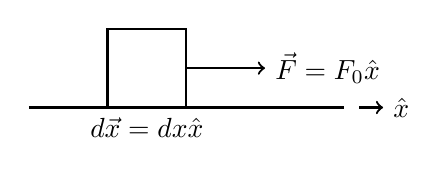
\begin{tikzpicture}
		\draw[thick] (0,0) -- (4,0);
		\draw[thick,->] (4.2,0) -- (4.5,0) node[anchor=west] {$\hat{x}$};
		\node[anchor=north] at (1.5,0) {$d\vec{x} = dx\hat{x}$};
		\draw[thick] (1,0) rectangle (2,1);
		\draw[thick,->] (2,0.5) -- (3,0.5) node[anchor=west] {$\vec{F} = F_{0}\hat{x}$};
	\end{tikzpicture}
\end{center}
\textbf{Total Energy} \\
The block can have kinetic energy, so its change in total energy is the difference of its final and initial kinetic energies. Its initial speed is 0 m/s, so
\[
\Delta E = K_{f}-K_{i} = \frac{1}{2}mv_{f}^{2} - \frac{1}{2}mv_{i}^{2} = \frac{1}{2}mv_{f}^{2}.
\]
Plugging in numbers, we obtain $\Delta E = 9000$ J. \\
\textbf{Distance} \\
By the work-energy theorem, $W_{\text{net,ext}} = \Delta E$, so if there is no friction and the winch is the only thing doing work, then we can calculate the distance $d$ from the work it did:
\[
W = \int_{0}^{d}\vec{F}\cdot d\vec{x} = F_{0} d = \Delta E = \frac{1}{2}mv_{f}^{2}.
\]
Solving for $d$ gives us $d = \frac{m}{2F_{0}}v_{f}^{2}$, and plugging in numbers gives us $d = 0.5$ m. \\
\textbf{Power} \\
We know how much energy the winch put into this endeavor, so all we need to find out is the time it took to move the block. For constant acceleration (which we have in this situation of constant force), we know $a = \frac{\Delta v}{\Delta t} = \frac{F_{0}}{m}$, so $\Delta t = \frac{v_{f}m}{F_{0}} = \frac{1}{6}$ s. This means that the power is
\[
P = \frac{\Delta E}{\Delta t} = \frac{F_{0}d}{v_{f}m/F_{0}} = \frac{F_{0}^{2}d}{v_{f}m}.
\]
Given what we know about the distance, this simplifies to
\[
P = \frac{F_{0}^{2}}{v_{f}m}\frac{m}{2F_{0}}v_{f}^{2} = \frac{F_{0}v_{f}}{2} = 54,000\text{ W}.
\]
For comparison, the light bulb in my desk lamp in my apartment consumes 9 W while on (this is much more efficient than an equivalently bright incandescent bulb, which would take about 60 W). This much power could light 6,000 desk lamps (or 900 if using an incandescent bulb)!
\end{TeacherMargin}
\begin{PresentSpace}
\vspace{-10pt}
\section*{L\Week-3: The Winch -- Part 1}
\vspace{-10pt}
A winch acts a constant force $F_{0}=18,000$ N on a metal block ($m=500$ kg) to accelerate it across level ground from rest to a final speed of $v_{f}=6$ m/s.
\begin{itemize}
	\item What is the block's change in total energy?
	\item How far did the winch move the block?
	\item How much power does this winch use?
\end{itemize}
\end{PresentSpace}
\newpage
\begin{TeacherMargin}
\noindent\textbf{Force} \\
To keep the block at constant speed, the winch must exert a force equal in magnitude to the force of gravity on the block:
\begin{center}
	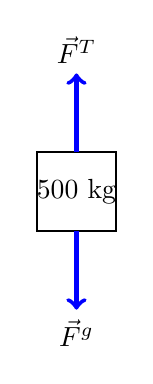
\begin{tikzpicture}
		\FBDbox{0,0}{0}{block}{500 kg}
		\FBDvectorXY{blocktcent}{0,1}{FT}
		\node[anchor=south] at (FTtip) {$\vec{F}^{T}$};
		\FBDvectorXY{blockbcent}{0,-1}{FG}
		\node[anchor=north] at (FGtip) {$\vec{F}^{g}$};
	\end{tikzpicture}
\end{center}
\[
F^{T} = F^{g} = mg \approx (500\text{ kg})(10\text{ m/s}^{2}) = 5000\text{ N}
\]
\textbf{Distance Lifted} \\
We know the speed of the block and how long it is in motion, so we can calculate its displacement directly from this:
\[
\Delta y = v\Delta t = (2\text{ m/s})(30\text{ s}) = 60\text{ m}.
\]
\textbf{Work}
\begin{align*}
	W & = \int_{y_{i}}^{y_{f}}\vec{F}\cdot d\vec{y} = \int_{y_{i}}^{y_{f}}\left(F\hat{y}\right)\cdot\left(dy\hat{y}\right) = \int_{y_{i}}^{y_{f}}Fdy \\
	& = F\Delta y = (5000\text{ N})(60\text{ m}) = 300,000\text{ J}
\end{align*}
Note that the speed is not changing, so the total energy of the block is not changing. That means $W_{\text{net,ext}}=\Delta E_{\text{total}} = 0$. Something else must be doing work to remove energy from the system! This is being done by gravity. \\
\textbf{Power} \\
The winch is transferring 300,000 J of energy over the course of 30 s, so the power is
\[
P = \frac{\Delta E}{\Delta t} = \frac{300,000\text{ J}}{30\text{ s}} = 10,000\text{ W}.
\]
This much power could light about 1,111 desk lamps (or about 166 if using an incandescent bulb)!
\end{TeacherMargin}
\begin{PresentSpace}
\vspace{-10pt}
\section*{L\Week-3: The Winch -- Part 2}
\vspace{-10pt}
You want to use the winch to lift the block into the air at a constant speed: $v=2$ m/s.
\begin{itemize}
	\item What force should you set the winch for?
	\item How far does the winch move the block from $t=0$ s to $t=30$ s?
	\item How much work does the winch do in $\Delta t = 30$ s?
	\begin{itemize}
		\item Is anything else doing work on the block?
	\end{itemize}
	\item How much power does the winch use now?
\end{itemize}
\end{PresentSpace}
\newpage
\begin{TeacherMargin}

\end{TeacherMargin}
\begin{PresentSpace}
\vspace{-10pt}
\section*{Energy Analysis}
\vspace{-10pt}
\begin{itemize}
	\item Understanding: Identify a system and the types of energy within the system.
	\item Calculating: Is your system's energy conserved or not? Once you know, use the work-energy theorem!
	\item Sensemaking: All the sensemaking strategies you have will work, but a new strategy is sometimes useful: Solve Multiple Ways.
	\begin{itemize}
		\item You have kinematics and force techniques at your disposal, so you can solve problems with these and compare their results to the results of your energy approach.
	\end{itemize}
\end{itemize}
\end{PresentSpace}
\newpage
\begin{TeacherMargin}
	
\end{TeacherMargin}
\begin{PresentSpace}
\section*{Main Ideas}
\begin{itemize}
	\item Energy is a powerful, ubiquitous concept that can help us solve a wide array of physics problems.
	\item Energy is a \textit{scalar}---it is not a vector.
	\item There are different forms of energy, and energy can be transferred between objects and between forms.
\end{itemize}
\end{PresentSpace}
\end{document}